% CSL7360 Assignment 2 report. Build:  python report/make_assets.py && cd report && tectonic report.tex
\documentclass[11pt,a4paper]{article}
\usepackage[margin=2.2cm]{geometry}
\usepackage[T1]{fontenc}
\usepackage{lmodern}
\usepackage{amsmath}
\usepackage{booktabs}
\usepackage{graphicx}
\usepackage{xcolor}
\usepackage{tikz}
\usetikzlibrary{positioning,arrows.meta,fit}
\usepackage[most]{tcolorbox}
\usepackage{enumitem}
\usepackage{float}
\usepackage[hidelinks]{hyperref}
\setlist{itemsep=2pt,topsep=4pt}

\newcommand{\CPUName}{Apple M3}
\newcommand{\OSName}{macOS-27.0.1-arm64-arm-64bit}
\newcommand{\TorchVersion}{2.15.0}
\newcommand{\TcpuMs}{3.67}
\newcommand{\TcpuN}{5,019}
\newcommand{\SdiskBytes}{337,026}
\newcommand{\SdiskMiB}{0.321}
\newcommand{\NParams}{299,489}
\newcommand{\CES}{0.6553}
\newcommand{\ValMiou}{0.8828}
\newcommand{\ValBFone}{0.6922}
\newcommand{\ValQ}{0.8256}
\newcommand{\ValN}{1,053}
\newcommand{\TeMiou}{0.7357}
\newcommand{\TeBFone}{0.5182}
\newcommand{\TeQ}{0.6705}
\newcommand{\TeN}{5,019}
\newcommand{\CapMiou}{pending}
\newcommand{\CapBFone}{pending}
\newcommand{\CapQ}{pending}
\newcommand{\CapN}{pending}
\newcommand{\TimePenalty}{0.0147}
\newcommand{\SizePenalty}{0.0080}
\newcommand{\CESCheck}{0.6553}
\newcommand{\TuneDefaultQ}{0.8199}
\newcommand{\TuneDefaultCES}{0.8011}
\newcommand{\TuneBestQ}{0.8256}
\newcommand{\TuneBestCES}{0.8067}
\newcommand{\TuneBestThr}{+0.6}
\newcommand{\TuneBestTTA}{off}
\newcommand{\TuneN}{1,053}
\newcommand{\LayoutContig}{3.63}
\newcommand{\LayoutCL}{43.34}
\newcommand{\TeShareIoULow}{7.1}
\newcommand{\TeShareIoUHigh}{6.0}
\newcommand{\TeMedianIoU}{0.658}
\newcommand{\HaveCaptured}{0}

\makeatletter\newcommand{\inputtable}[1]{\@@input #1 }\makeatother  % \input that works inside tabular
\newcommand{\YourName}{Neeraj Kumar}
\newcommand{\RollNo}{B23CS1044}

\title{\textbf{CSL7360 Computer Vision -- Assignment 2}\\[2pt]
       \large Cost-Efficient Segmentation under a Compute Budget (Track B: tiny FCN)}
\author{\YourName{} (\RollNo)}
\date{}

\begin{document}
\maketitle

\begin{tcolorbox}[colback=yellow!8,colframe=orange!70!black,title=Provenance of the results in this version of the report]
\textbf{Code.} Everything described here (data preparation, network, training, export, timed pipeline,
\texttt{predict.py}, metrics, timing, evaluation, tuning and figures) is this project's own code.

\textbf{Weights.} The full training run of my own model (\texttt{src/train.py}) has not been completed yet.
The network weights evaluated below are the \emph{reference model} distributed with the course sample code,
trained by that code's author. They were converted into this project's parameter format with
\texttt{src/convert\_reference.py}; this is possible because both networks share the same layer structure.
The converted model reproduces the reference pipeline's masks pixel for pixel.
All numbers below were then measured with this project's code on my laptop (\CPUName).

\textbf{Own photos.} Pending. The captured-photo row and Section~\ref{sec:captured} are filled in automatically
once my photos and masks are in \texttt{captured/}.
\end{tcolorbox}

%------------------------------------------------------------------------------------------
\section{Final results}
\begin{table}[H]
\centering
\begin{tabular}{lrccc}
\toprule
Set & Photos & mIoU & Boundary F1 & $Q$ \\
\midrule
\inputtable{generated/tab_results.tex}
\bottomrule
\end{tabular}
\\[6pt]
\begin{tabular}{ccc}
\toprule
$T_\text{CPU}$ (DUTS-TE, 1 thread) & $S_\text{disk}$ & \textbf{CES} (on DUTS-TE) \\
\midrule
\TcpuMs{} ms & \SdiskBytes{} B (\SdiskMiB{} MiB) & \textbf{\CES} \\
\bottomrule
\end{tabular}
\caption{Results of the deployed pipeline (reference weights, this project's pipeline and tuning).
$Q = 0.70\,\text{mIoU} + 0.30\,\text{BF1}$. CES $= Q_\text{TE}\,[1 - \TimePenalty - \SizePenalty] = \CESCheck$.}
\label{tab:results}
\end{table}

\begin{itemize}
  \item \textbf{CPU:} \CPUName, \OSName, PyTorch \TorchVersion, one thread.
        $T_\text{CPU}$ is the total \texttt{time.process\_time()} over all \TcpuN{} DUTS-TE photos divided by their number,
        after one untimed warm-up run.
  \item \textbf{Split:} DUTS-TR (10,553 photos) is split into \textbf{9,500 training} and \textbf{\ValN{} validation}
        photos with a fixed seed. Validation uses the split the reference weights were trained with, so no
        validation photo was seen in training. My own code's default split (seed 0) is 9,498 / 1,055.
  \item \textbf{DUTS-TE} was used only for the final table, the official timing and the failure analysis,
        never for training, tuning or model selection.
\end{itemize}

%------------------------------------------------------------------------------------------
\section{Method}
\subsection{Data}
Every photo is resized to $256\times256$ with \texttt{cv2.INTER\_AREA} and every mask with
\texttt{cv2.INTER\_NEAREST}; a mask pixel is object if its value is at least 128 (\texttt{src/data.py}).
The resized sets are cached once as memory-mapped \texttt{uint8} arrays. Photos stay in OpenCV's BGR order end
to end, so the timed pipeline needs no colour conversion.

\subsection{Network (\texttt{src/model.py})}
A small fully convolutional U-Net built from depthwise separable convolutions (Fig.~\ref{fig:arch}).
The deployed configuration has \NParams{} parameters and works on a $128\times128$ copy of the photo.

\begin{figure}[H]
\centering
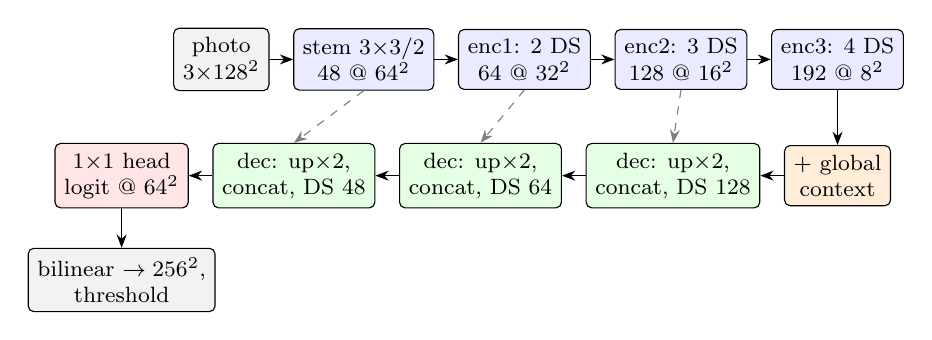
\begin{tikzpicture}[
  blk/.style={draw,rounded corners=2pt,minimum height=7mm,align=center,font=\footnotesize,fill=#1},
  blk/.default=blue!8, >=Stealth, node distance=3mm]
  \node[blk=gray!10] (in) {photo\\$3{\times}128^2$};
  \node[blk,right=of in] (stem) {stem 3$\times$3/2\\48 @ $64^2$};
  \node[blk,right=of stem] (e1) {enc1: 2 DS\\64 @ $32^2$};
  \node[blk,right=of e1] (e2) {enc2: 3 DS\\128 @ $16^2$};
  \node[blk,right=of e2] (e3) {enc3: 4 DS\\192 @ $8^2$};
  \node[blk=orange!15,below=7mm of e3] (ctx) {+ global\\context};
  \node[blk=green!10,left=of ctx] (d2) {dec: up$\times$2,\\concat, DS 128};
  \node[blk=green!10,left=of d2] (d1) {dec: up$\times$2,\\concat, DS 64};
  \node[blk=green!10,left=of d1] (d0) {dec: up$\times$2,\\concat, DS 48};
  \node[blk=red!10,left=of d0] (head) {1$\times$1 head\\logit @ $64^2$};
  \node[blk=gray!10,below=5mm of head] (out) {bilinear $\to256^2$,\\threshold};
  \draw[->] (in)--(stem); \draw[->] (stem)--(e1); \draw[->] (e1)--(e2); \draw[->] (e2)--(e3);
  \draw[->] (e3)--(ctx); \draw[->] (ctx)--(d2); \draw[->] (d2)--(d1); \draw[->] (d1)--(d0); \draw[->] (d0)--(head);
  \draw[->] (head)--(out);
  \draw[->,dashed,gray] (e2.south)--(d2.north); \draw[->,dashed,gray] (e1.south)--(d1.north);
  \draw[->,dashed,gray] (stem.south)--(d0.north);
\end{tikzpicture}
\caption{Network. DS = depthwise separable block (depthwise 3$\times$3, BN, ReLU, pointwise 1$\times$1, BN,
residual add when shapes match, ReLU); the first block of every encoder stage has stride 2.
Dashed arrows are U-Net skip connections (concatenation).}
\label{fig:arch}
\end{figure}

\begin{itemize}
  \item \textbf{Encoder} shrinks the image by 16 in four steps. Depthwise separable blocks keep the cost low.
  \item \textbf{Global context:} the mean of the deepest feature map goes through a 1$\times$1 conv and is added to
        every position, so each pixel knows about the whole image (which object is the main one) at almost no cost.
  \item \textbf{Decoder:} bilinear $\times2$ upsampling, concatenation with the encoder skip of the same size, one DS block.
  \item \textbf{Head:} a 1$\times$1 conv gives one object logit per pixel at $64\times64$, bilinearly upsampled to
        $256\times256$. One logit with binary cross entropy is the two-class pixel-wise cross entropy.
\end{itemize}

\subsection{Training (\texttt{src/train.py})}
\begin{itemize}
  \item \textbf{Loss:} pixel-wise binary cross entropy plus soft Dice. Pixels within 2\,px of the true outline get
        a higher BCE weight (\texttt{-{}-boundary-weight}), since BF1 only rewards outlines inside a 5$\times$5 window.
  \item \textbf{Optimiser:} AdamW (lr $3\cdot10^{-3}$, weight decay $10^{-4}$), one warm-up epoch, cosine decay,
        batch 32, optional exponential moving average of the weights (\texttt{-{}-ema}).
  \item \textbf{Augmentation (on the training device):} random zoom, rotation, shift and horizontal flip (the
        same warp for photo and mask); brightness, contrast, saturation, per-channel colour cast (daylight vs tube
        light), gamma, occasional blur and sensor noise.
  \item \textbf{Hardware:} the Mac GPU (Apple MPS), about 40\,s per epoch for this network size.
  \item \textbf{Model selection:} the epoch with the best validation $Q$ is kept; candidate models are ranked by
        validation CES with \texttt{src/compare.py}.
\end{itemize}
The reference weights were trained with the same kind of recipe (BCE + Dice with boundary weighting, AdamW with
cosine decay, 60 epochs). Their training log is in Fig.~\ref{fig:curve}.

\begin{figure}[H]
\centering
\IfFileExists{figures/curve_reference.png}{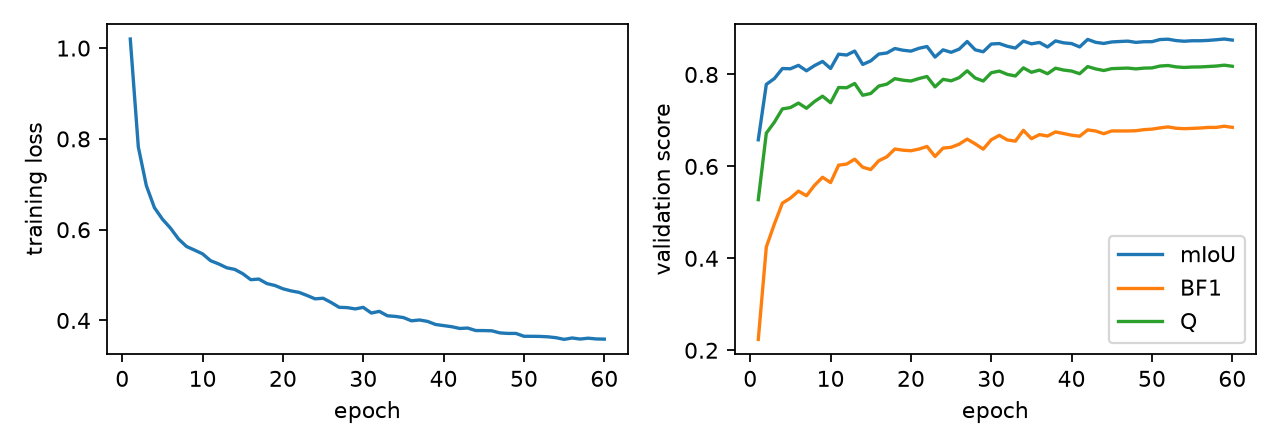
\includegraphics[width=0.9\linewidth]{figures/curve_reference.png}}{\fbox{pending}}
\caption{Training log of the reference weights (from the sample code's \texttt{results/train\_final.json}, plotted by
\texttt{report/make\_assets.py}). The best validation $Q$ is at epoch 59 of 60.}
\label{fig:curve}
\end{figure}

\subsection{Deployment (\texttt{src/export.py}, \texttt{src/weights\_io.py})}
\begin{itemize}
  \item Every BatchNorm is folded into its convolution and the $1/255$ input scaling is folded into the stem,
        so the network takes the raw \texttt{uint8} photo.
  \item Convolution weights are stored as \texttt{int8} with one \texttt{float32} scale per output channel, and biases
        as \texttt{float16}, in a plain \texttt{torch.save} file without extra compression. The file also stores
        the decision threshold and the test-time-augmentation flag, so every learned value lives in it.
        Weights are cast back to \texttt{float32} once at load time, which is not timed.
\end{itemize}

%------------------------------------------------------------------------------------------
\section{Keeping it fast}
The timed part of \texttt{src/pipeline.py} starts with the $256\times256$ photo in memory and ends with the
$256\times256$ mask of 0s and 1s in memory. It runs on one thread: the four thread variables are set to 1 before
NumPy, OpenCV or PyTorch are imported, then \texttt{cv2.setNumThreads(1)} and \texttt{torch.set\_num\_threads(1)}
are called.
\begin{itemize}
  \item \textbf{Low working resolution:} the network sees a $128\times128$ copy and predicts at $64\times64$.
        Only the single-channel logit is upsampled to full size, with \texttt{cv2.resize}.
  \item \textbf{Cheap layers:} depthwise separable convolutions, with BN and input scaling folded in.
  \item \textbf{No Python overhead:} the network is traced and frozen with TorchScript at load time and warmed up
        before timing starts.
  \item \textbf{Memory layout:} on this Apple M3, the \texttt{channels\_last} layout that helps on x86 makes the
        pipeline about 12$\times$ slower (\LayoutCL{} ms vs \LayoutContig{} ms per photo on validation photos), so
        the default contiguous layout is used.
\end{itemize}

\begin{table}[H]
\centering
\begin{tabular}{lr}
\toprule
Stage & ms / photo \\
\midrule
\inputtable{generated/tab_stages.tex}
\bottomrule
\end{tabular}
\caption{Where the time goes (validation photos, 1 thread). The network is almost all of it.}
\label{tab:stages}
\end{table}

The budget is generous. At $Q\approx0.66$, one extra millisecond of $T_\text{CPU}$ costs about $0.0026$ CES and
one extra MiB of parameters about $0.0165$, while $+0.01$ mIoU on DUTS-TE gains about $0.0068$ and $+0.01$ BF1
about $0.0029$. Quality $Q$ therefore matters far more than speed, as long as the file stays small.

\begin{table}[H]
\centering\small
\begin{tabular}{llrrrrr}
\toprule
Candidate & widths / depths & input & params & bytes & ms & ms, TTA \\
\midrule
\inputtable{generated/tab_bench.tex}
\bottomrule
\end{tabular}
\caption{Single-thread CPU time of candidate architectures with random weights (\texttt{src/bench.py}).
\texttt{r128\_w48} is the deployed configuration.}
\label{tab:bench}
\end{table}

%------------------------------------------------------------------------------------------
\section{Tuning on validation}
With the weights fixed, I tuned the two inference settings stored in the parameter file on the \TuneN{}
validation photos (\texttt{src/tune\_deployed.py}): the logit threshold, and flip test-time augmentation
(averaging the logits of the photo and its mirror image, run as one batch of two).
Each setting is scored by validation CES, with time measured on 500 validation photos.

\begin{table}[H]
\centering\small
\begin{tabular}{ccccccc}
\toprule
Flip TTA & threshold & mIoU & BF1 & $Q$ & ms & val CES \\
\midrule
\inputtable{generated/tab_tuning.tex}
\bottomrule
\end{tabular}
\caption{Validation sweep (every 0.2 shown; the search used steps of 0.1). The best setting, in bold
(threshold \TuneBestThr, flip TTA \TuneBestTTA), gives validation CES \TuneBestCES{} vs \TuneDefaultCES{} for
the default (threshold 0, no TTA), and is the one deployed.}
\label{tab:tuning}
\end{table}

%------------------------------------------------------------------------------------------
\section{Own photos}\label{sec:captured}
\ifnum\HaveCaptured=1
Fig.~\ref{fig:captured} shows every photo with the true mask (green, left) and the predicted mask (magenta, right)
as semi-transparent overlays.
\begin{figure}[H]
\centering
\includegraphics[width=0.75\linewidth]{figures/captured_overlays.png}
\caption{Own photos: true (left) vs predicted (right) masks, with per-photo object IoU and BF1.}
\label{fig:captured}
\end{figure}
\else
\textit{Pending.} My 5--10 phone photos (covering at least three of: indoor and outdoor, daylight and tube light,
near and far, clutter, partial occlusion) go in \texttt{captured/original/}. Masks are drawn on the resized photos
with \texttt{src/annotate.py}. Running \texttt{python -m src.evaluate -{}-sets captured},
\texttt{python -m src.figures captured} and \texttt{python report/make\_assets.py} fills in this section and the
last row of Table~\ref{tab:results}.
\fi

%------------------------------------------------------------------------------------------
\section{Failure analysis}
% Failure analysis (hand-written; the cases were chosen by looking at report/figures/worst_te.png)
Most photos are segmented reasonably well (median object IoU on DUTS-TE \TeMedianIoU), but the distribution
has a long tail: \TeShareIoULow\% of DUTS-TE photos have object IoU below 0.1, which means the network picked
the wrong region entirely (Fig.~\ref{fig:iouhist}). Fig.~\ref{fig:failures} shows four such cases from DUTS-TE,
all with IoU 0.

\begin{figure}[H]
\centering
\IfFileExists{figures/iou_hist.png}{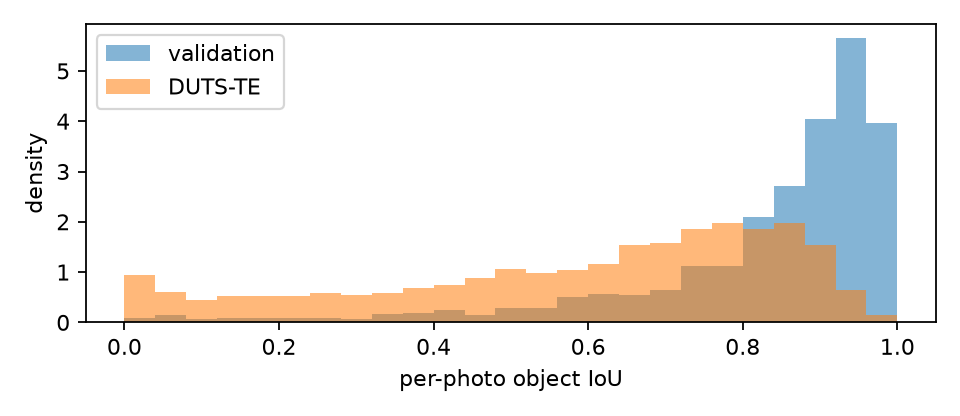
\includegraphics[width=0.62\linewidth]{figures/iou_hist.png}}{\fbox{pending}}
\caption{Per-photo object IoU on validation and DUTS-TE. DUTS-TE has many more near-zero failures.}
\label{fig:iouhist}
\end{figure}

\begin{figure}[H]
\centering
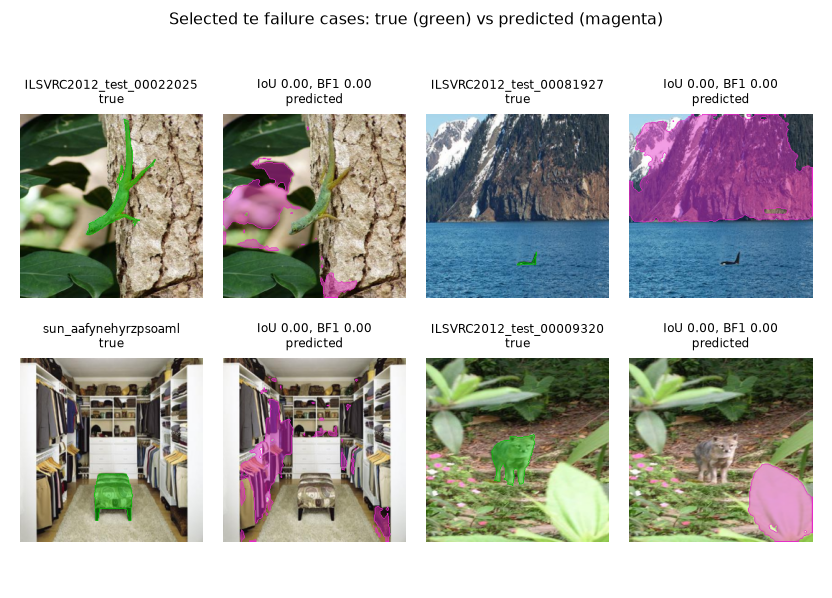
\includegraphics[width=0.92\linewidth]{figures/picked_te.png}
\caption{Four DUTS-TE failures (true mask green, prediction magenta).}
\label{fig:failures}
\end{figure}

\begin{enumerate}
  \item \textbf{Camouflage (lizard on bark, top left).} The green lizard has almost the same colour as the leaves and
        the same contrast as the bark texture. The network instead marks the large, blurred green leaf in the
        foreground. The lizard's thin legs and tail are 1--2 pixels wide at the network's $64\times64$ output, so
        even a correct detection would be hard to outline.
        \emph{Likely cause:} low colour and texture contrast between object and background, plus the coarse output.
  \item \textbf{Small, far object (orca, top right).} The orca covers well under 1\% of the photo, about 5 pixels
        across in the $128\times128$ input. The network segments the large, high-contrast mountain instead.
        \emph{Likely cause:} a small object. The global-context branch and the training data push the network
        towards large regions that stand out, and the low input resolution removes most of the small object's detail.
  \item \textbf{Clutter (walk-in closet, bottom left).} The annotated object is the ottoman in the centre, but the
        scene is full of clothes, shoes and shelves that are each just as distinctive. The network marks scattered
        pieces of the clothing and misses the ottoman, whose pattern blends with the rug.
        \emph{Likely cause:} a cluttered background with many candidate objects. Without enough context the network
        cannot tell which one the annotator meant.
  \item \textbf{Defocused foreground (kitten in plants, bottom right).} A large, bright, out-of-focus leaf at the
        bottom-right corner is predicted as the object, while the small grey kitten in the middle of the photo is
        missed. \emph{Likely cause:} a small, low-contrast object behind distracting foreground blur, which acts like
        partial occlusion.
\end{enumerate}

The validation failures (Fig.~\ref{fig:worstval}) show the same patterns: small objects (an insect on a tree trunk,
a bird on roof tiles) and camouflage (a scorpion lit in blue). They also show a further cause, \textbf{annotation
ambiguity}: in the savanna photo the ground truth marks the herd of zebras, but the lone tree is just as plausible
a ``main object'', and in the photo of a person holding a pretzel only the pretzel is marked. Such photos cap the
achievable score whatever the method.

\begin{figure}[H]
\centering
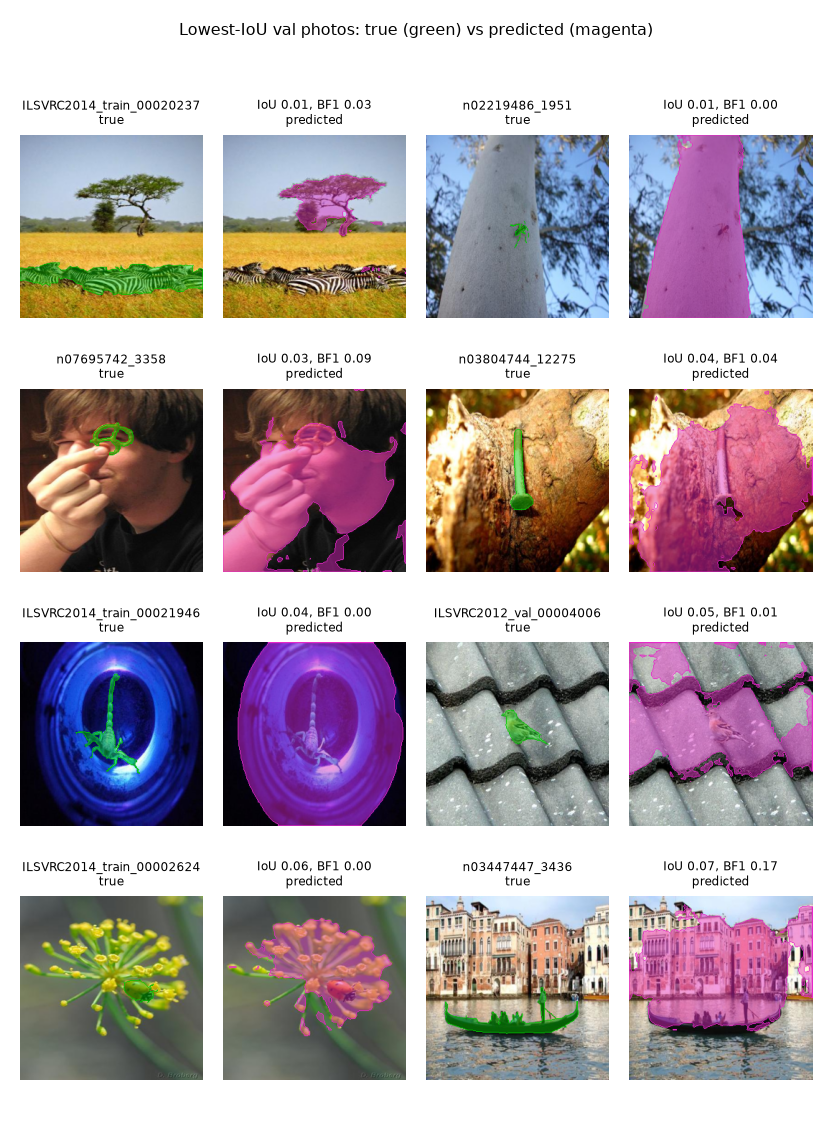
\includegraphics[width=0.85\linewidth]{figures/worst_val.png}
\caption{The eight lowest-IoU validation photos.}
\label{fig:worstval}
\end{figure}

These cases suggest specific fixes for my own training runs: zoom-out augmentation and a finer output (helping
small objects), a deeper or dilated context block (helping clutter), and colour and blur augmentation (helping
camouflage and defocus).


%------------------------------------------------------------------------------------------
\section{Generalisation}
Validation $Q$ is \ValQ{} but DUTS-TE $Q$ is \TeQ. The validation photos come from the same pool as the training
photos, while DUTS-TE contains many harder photos: clutter, several candidate objects, and small or camouflaged
objects (Section~6 and Fig.~\ref{fig:iouhist}).
The drop is larger for BF1 (\ValBFone{} $\to$ \TeBFone) than for mIoU (\ValMiou{} $\to$ \TeMiou): on harder photos
the coarse $64\times64$ prediction misses fine outlines first. The changes most likely to close the gap are the
ones planned for my own training runs: more context at the deepest level, a stronger boundary loss, weight EMA,
and augmentation that zooms out further and creates multi-object scenes.

%------------------------------------------------------------------------------------------
\section{Rules compliance}
\begin{itemize}
  \item Only Python's standard library, PyTorch, NumPy, OpenCV (I/O, resizing, drawing in the annotation tool) and
        Matplotlib are used. There are no pretrained weights from any library, and no library code for segmentation,
        clustering, morphology, connected components or metrics. Boundaries use shifted-tensor comparisons, and the
        5$\times$5 window test uses \texttt{F.max\_pool2d}; both are checked against a brute-force implementation
        (\texttt{tests/test\_metrics.py}).
  \item The timed pipeline runs on the CPU with one thread and no extra processes, and every learned value
        (weights, threshold, TTA flag) is in \texttt{weights/model.pt} (\SdiskBytes{} bytes, plain \texttt{torch.save}).
  \item \texttt{python predict.py -{}-image photo.jpg -{}-out mask.png} saves a 0/255 mask and prints exactly the two
        lines \texttt{T CPU ms} and \texttt{S disk bytes}.
\end{itemize}

\end{document}
